\begin{figure}
	\centering
	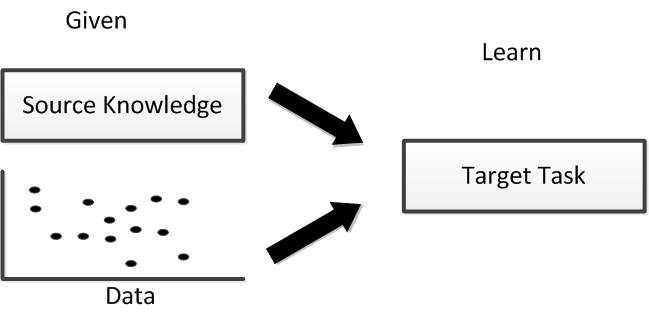
\includegraphics[scale =.7]{relatedwork/fig/transfer.png}
	\caption{Apart from the standard machine learning, transfer learning can leverage the information from an additional source: knoweldge from one or more related tasks.}
\end{figure}

Traditional machine learning algorithms try to build the classifiers from a set of training data and apply to the test data with the same distribution to the training data. In contrast, transfer learning attempts to change this by transfer the learned knowledge from one or several tasks (called \textbf{source tasks}) to improve a related new task (called \textbf{target task}). According to the situations of the source and target tasks, transfer learning can be categorized as 3 types: inductive transfer learning, transductive transfer learning and {unsupervised transfer learning}. On the other hand, from the types of the source knowledge, transfer learning can be classified as: instance transfer, feature representation transfer and parameter transfer. 

% Table generated by Excel2LaTeX from sheet 'Sheet1'
\begin{table}[htbp]
	\centering
	\caption{Categories of our learning scenarios}
	\begin{tabular}{|c|c|c|}
		\hline
		& Situation of Task     & Source Knowledge \\
		\hline
		Learning New Categories & Inductive Transfer & \multirow{2}[0]{*}{Parameter Transfer} \\
		\cline{1-2}
		Domain Adaptation & Transductive Transfer &  \\
		\hline
	\end{tabular}%
\end{table}%


\subsection{Types of Transfer Learning from the Situations of Tasks}
Transfer learning can be categorized into 3 sub-settings: \textbf{inductive transfer learning, transductive transfer learning} and \textbf{unsupervised transfer learning} based on the different situations of the source and target domains and tasks. \cite{pan2010survey}. We compared the differences of these three sub-categories and show them in Table \ref{tab:related:transfersetting}. 

\begin{table}[htbp]
	\centering
	\caption{Relationship between traditional machine learning and different transfer learning settings}
	\begin{tabular}{|c|c|c|c|}
		\hline
		\multicolumn{2}{|c|}{Learning settings} & Source target domain & Source target task \\
		\hline
		\multicolumn{2}{|c|}{Traditional machine learning} & the same & the same \\\hline
		\multirow{3}{*}{Transfer learning} & \textbf{Inductive transfer learning} & the same & different but related \\\cline{2-4}
		& Unsupervised transfer learning & different but related & different but related \\\cline{2-4}
		& Transductive transfer learning & different but related & the same \\\hline    
	\end{tabular}%
	\label{tab:related:transfercmp}%
\end{table}%

\begin{table}[htbp]
	\centering
	\caption{Various settings of transfer learning}
	\begin{tabular}{|c|C{4cm}|c|c|}
		\hline
		& Related areas & Source data & Target data \\
		\hline
		\multirow{2}[4]{*}{Inductive transfer learning} & self-taught learning & unlabeled & labeled \\\cline{2-4}
		& multi-task learning & labeled & labeled \\\hline
		Transductive transfer learning& \textbf{domain adaptation}, Sample selection bias & labeled & labeled/unlabeled \\\hline
		Unsupervised transfer learning &       & unlabeled & unlabeled \\
		\hline
	\end{tabular}%
	\label{tab:related:transfersetting}%
\end{table}%

\subsection{Types of Transfer Learning from the Aspect of Source Knowledge}
According to the type of the source knowledge comes from, transfer learning can be split into 3 major streams: instance transfer, feature representation transfer and parameter transfer.

The core idea of instance transfer learning is to select some useful data from the source task to help learning the target task. Dai et al. \cite{dai2007boosting} propose a method (called TrAdaBoost) that can select the most useful examples from the source task as the additional training examples for the target task. These useful examples are iteratively re-weighted according to the classification results of some base classifiers. Jiang et al. \cite{jiang2007instance} proposed a method that can ignore the "misleading" examples from the source data based on the conditional probabilities on the source task $P(y_t|x_t)$ and target task $P(y_s|x_s)$. Liao et al. \cite{liao2005logistic} proposed a active learning method that selects and labels the unlabeled data from the target data with the help of the source data. Ben-David et al. \cite{ben2010theory} provided a theoretical analysis the lowest target test error for different source data combination strategies when the source data is large and target training set is small.   

Feature representation transfer aims to find a good feature representations to reduce the gap between the source and target domains. According to the size of labeled examples in the source data, feature representation transfer consists of two approaches: supervised feature construction and unsupervised feature construction. When the source data are labeled, supervised feature transfer learning is used to find the feature representations shared in related tasks to reduce the difference between the source and target tasks. Evgeniou et al. \cite{evgeniou2007multi} proposed a method that can learn sparse low-dimension feature representations that can share between different tasks. Jie et al. \cite{jie2011multiclass} reconstructed the feature representations for the target data by using the outputs of the source models as the auxiliary feature representations. In unsupervised feature representation transfer learning, Daume III \cite{daume2009frustratingly} proposed a simple feature reconstruction method for both source and target data so that source and target data are triple augmented and a SVM model is trained on both source and target data.

Parameter transfer assumes that there should be some parameters or prior distribution of the hyperparameters in the individual models of related tasks. Most of the approaches are designed under the multi-task learning scenario. Therefore, in this thesis, we also focus on the parameter transfer approach to leverage the knowledge from the source data. In parameter transfer learning, there are three major frameworks: a regularization framework, a Bayesian framework and a neural network framework.
\begin{figure}
	\centering
	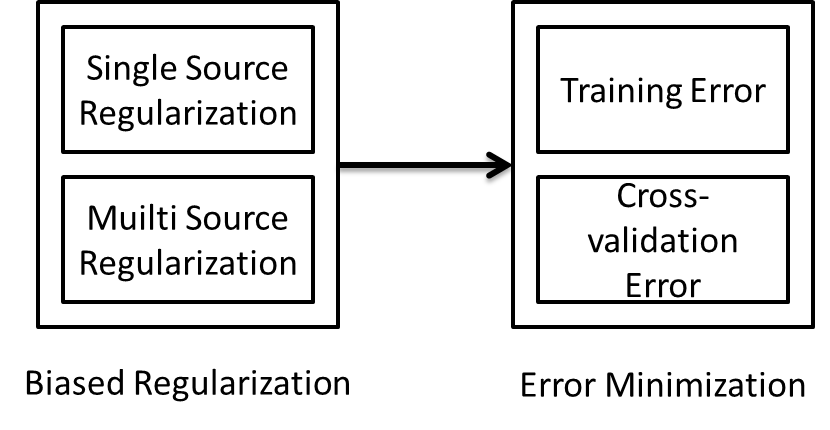
\includegraphics[scale =1]{relatedwork/fig/parameters.png}
	\caption{Two steps for parameter transfer learning. In the first step multi-source and single source combination are usually used to generate the regularization term. The hyperplane for the transfer model can be obtained by either minimizing training error or cross-validation error on the target training data.}
\end{figure}
\begin{itemize}
	\item Regularization framework: In the regularization framework, some researchers propose to transfer the parameters of the SVM following the assumption that the hyperplane for the target task should be related to the hyperplane of the source models. Evgeniou et al. \cite{evgeniou2004regularized} proposed an idea that the hyperplane of the SVM for the target task should be separate into two terms: a common term shared over tasks and a specific term related to the individual task. Inspired by this idea, some researchers propose different strategies to combine these two terms for transfer learning \cite{aytar2011tabula} \cite{tommasi2010safety} \cite{yang2007cross}. Most of these work contains two steps. In the first step, a SVM objective function with a biased regularization term for the target model is built. Then another objective function is built to reduce the empirical error of the target model on the target data.
	\item Neural network framework. In neural network framework, the idea is to use the parameters of a CNN pre-trained from a very large dataset as an initialization to reduce the target data bias when it is small. Yosinski et al. \cite{yosinski2014transferable} show that the high level layer parameters are more related to a specific task while the low level layer ones are more general and transferable. This framework is widely used for image recognition task. By re-using and fine-tuning the parameters of some layers in the pre-trained model, the bias of the target task can be greatly alleviated \cite{Chatfield14} \cite{hoffman2013one}  \cite{zeiler2014visualizing} \cite{NIPS2014_Zhou}. 
	\item Bayesian framework. In Bayesian framework, one or several posterior probabilities of the source data or parameters of the source model can be used to generate a prior probability for the target task. With this prior probability, a posterior probability for the target task can be obtained with the target data.
	Li et al. \cite{fei2006one} used a prior probability density function to model the knowledge from the source and modify it with the data from target to generate posterior density for detection and recognition. 
	Rosenstein et al. \cite{rosenstein2005transfer} used hierarchical Bayesian method to estimate the posterior distribution for all the parameters and the overall model can decide the similarities of the source and target tasks. 
\end{itemize}

\subsection{Special Issues in Avoiding Negative Transfer}
In transfer learning, for a given target task, the performance of a transfer method depends on two aspects: the quality of the source task and the transfer ability of the transfer algorithm. The quality of the source task refers to how the source and target tasks are related. If there exists a strong relationship between the source and target, with a proper transfer method, the performance in the target task can be significantly improved. However, if the source and target tasks are not sufficiently related, despite of the transfer ability of the transfer algorithm, the performance in the target task may fail to be improved or even decrease. In transfer learning, negative transfer refers to the degraded performance compare to a method without using any knowledge from the source \cite{pan2010survey}. How to avoid negative transfer is still an open question for researchers. 
For example, we can use a teacher-student diagram to illustrate the procedure of transfer learning. The student (target model) would like to learn the new knowledge (target task) with the assistance of a teacher (source knowledge). If the teacher can provide helpful knowledge (related knowledge), the student can learn the new knowledge very quickly (positive transfer). If the teacher can only provide useless knowledge, the student could not learn the new knowledge effectively or even get confused (negative transfer).

\begin{figure}
	\centering
	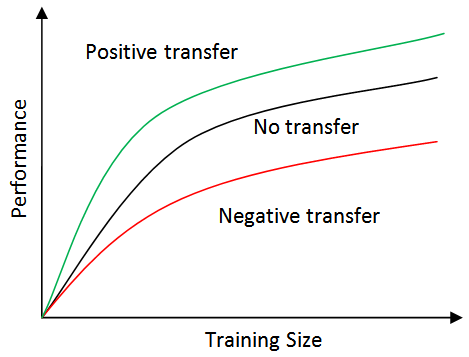
\includegraphics[scale=.7]{relatedwork/fig/negative.png}
	\caption{Positive transfer VS Negative transfer.}
\end{figure}

Another important aspect that affect the learning performance is the transfer ability of the algorithm used for the target task. An ideal transfer algorithm would be able to produce positive transfer on related tasks while avoiding negative transfer on unrelated tasks. However, in practice, it is not easy to achieve these two goals simultaneously. Approaches that can avoid negative transfer often bring some affects on positive transfer due to their caution. On the other hand, approaches using aggressive transfer strategies often have little or no protection against negative transfer \cite{torrey2009transfer}. Even though voiding negative transfer is an important issue in transfer learning, how to avoid negative transfer has not been widely addressed \cite{lu2015transfer} \cite{pan2010survey}. Previous work show suggest that negative transfer can be alleviated through 3 approaches \cite{torrey2009transfer}: 
\begin{itemize}
	\item Rejecting unrelated source information. A important approach to avoid negative transfer is to recognize and reject unrelated and harmful source knowledge. The goal of this approach is to minimize the impact of the unrelated source, so that the transfer model performs no worse than the learned model without transfer. Therefore, in some extreme situation, the transfer model is allowed to completely ignore the source knowledge. 
	Torrey et al. \cite{torrey2005using} proposed a method using advice-taking algorithm to reject the unrelated source knowledge. 
	Rosenstein et al. \cite{rosenstein2005transfer} presented an approach that use naive Bayes classifier to detect and reject the unrelated source.
	\item Choosing correct source task. When the source knowledge come from more than one candidate source, it is possible for the transfer model to select the best source knowledge of the candidates. In this scenario, leverage the knowledge from the best candidate may be effective against negative transfer as long as the best source knowledge is sufficiently related. 
	Talvitie et al. \cite{talvitie2007experts} proposed a method that can iteratively evaluate the candidate sources through a trail-and-error approach and select the best one to transfer. Kuhlmann et al. \cite{kuhlmann2007graph} constructed a kernel function from certain sources for the target task by estimating the bias from a set of candidate sources whose relationship to the target task is unknown.
	\item Measuring task similarity. To achieve a better transfer performance, it is reasonable for a transfer method to transfer the knowledge from multiple sources instead of just choosing a single source. In this approach, some methods try to involve all the source knowledge without considering the explicit relationship between the source and target. The other methods try to model the relationships between the source and target tasks and use the information as a part of their transfer methods which can significantly reduce the affect of negative transfer.
	Bakker et al. \cite{bakker2003task} proposed a method to provide guidance on how to avoid negative transfer by using clustering and Bayesian approach to estimate the similarities between the target task and multiple source tasks.
	Tommasi et al. \cite{tommasi2014learning} constructed the transfer model by using some transfer parameters to measure the relationships between each source and the target tasks and the transfer parameters are optimized by minimizing the cross-validation error of the transfer model. Similar approaches can be found in \cite{jie2011multiclass} \cite{kuzborskij2013n}.
	Kuzborskij et al. \cite{kuzborskij2013stability} provided some theoretical analysis of transfer learning and show that regularized least square SVM with truncation function and leave-one-out cross-validation for source task measurement can reduce negative transfer even though the training data of the target task is relatively small.
\end{itemize}

Here we can see that most of the previous approaches focus on measuring the similarity of the source and target tasks, i.e. try to assign the most related source tasks to the target one through various of metrics and use aggressive transfer algorithm to exploit the source knowledge. Just a few work \cite{kuzborskij2013stability} \cite{tommasi2010safety} addressed the problem that a sophisticated transfer algorithm should be designed to better exploit the source knowledge as well as avoid negative transfer. Therefore, in this thesis, we mainly focus on how to design a better transfer algorithm for transfer learning while certain source knowledge is assigned. 

To summarize, in this section, we provided an overview of the categories of transfer learning from two different views. From the relationships of the tasks, our two transfer learning scenarios belong to inductive transfer and transductive transfer learning respectively. In this thesis, we assume that we are not able to access to the source data, therefore, from the aspect of source knowledge, we use parameter transfer for both scenarios. In this thesis, without observing any source data, it is difficult to measure the relationship between the source and target tasks. Therefore, avoiding negative transfer is also an important part we have to consider. Finally, we reviewed some methods that cab alleviate negative transfer.

\section{Related Work in Hypothesis Transfer Learning}
The main topic of this thesis is to investigate the problem of visual transfer learning under the HTL setting. Therefore, in this section, we show some work related to this topic and this thesis. We first review some work in fine-tuning the deep neural networks for inductive transfer learning related to our work in chapter \ref{sec:cnn}. Then we discuss some methods in hypothesis transfer learning, which is related to our work in chapter \ref{sec:pakdd}. The related work in chapter \ref{sec:aaai} is reviewed at last.

\subsection{Fine-tuning the Deep Net}
Since Deep Convolutional Neural Networks (CNNs) became the most powerful algorithm in object recognition task, fine-tuning the deep CNNs has become a popular and effective way to transfer the knowledge between different visual recognition tasks. The intuition of fine-tuning the deep CNNs for transfer learning is that low-level features, such as edges and lines, are universal for object recognition while high-level features, which are the combinations of the low-level features, are more specific for the designed task. Because deep CNNs can learn hierarchical features, from abstract low-level features to detailed high-level ones, by changing the combinations of the low-level features in the pre-trained deep CNNs, the high-level features can be learned effectively for the new recognition task \cite{farabet2013learning}.

\begin{figure}
	\centering
	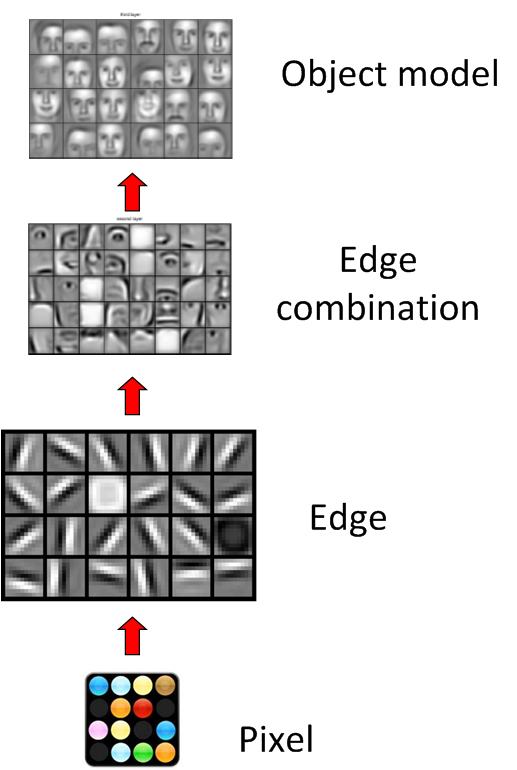
\includegraphics[scale=.7]{relatedwork/fig/hierachy}
	\caption{Hierarchical Features of Deep Convolutional Neural Networks for face recognition.}
\end{figure}

Applying the pre-trained model from ImageNet dataset on other object recognition benchmark datasets shows some impressive results. Zeiler et al.  \cite{zeiler2014visualizing} applied their pre-trained model on Caltech-256 with just 15 instances per class and improved the previous state-of-the-art in which about 60 instances were used, by almost 10\%.
Chatfield et al.  \cite{Chatfield14} used their pre-trained model on the VOC2007 dataset and outperformed the previous state-of-the-art by 0.9\%.
Agrawal et al. \cite{agrawal2014analyzing} show that even in the mid-level features, there are some grandmother cells, which can capture the high-level features of specific objects. Hoffman et al. \cite{hoffman2013one} show that even with one labeled example per class, it is possible to fine-tune the pre-trained deep CNNs and obtain a good classifier for some new recognition tasks. Zhou et al. \cite{NIPS2014_Zhou} provided the state-of-the-art performance using the deep features on some scene benchmarks by fine-tuning the deep CNNs. Yosinski et al. \cite{yosinski2014transferable} investigated the transferability of the layers in deep CNNs and show that the target task can be benefited from pre-training even though the source and target tasks are distant. 

In this thesis, we also use the pre-trained deep CNNs to learn new categories for food recognition and investigate the affects of each layer in deep CNNs for knowledge transfer in chapter \ref{sec:cnn}.

\subsection{Hypothesis Transfer Learning with SVMs}
In this part, We will introduce the framework of \textbf{Hypothesis Transfer Learning} (HTL). HTL is proposed to effective utilize the source knowledge, especially the source model, while we are not able to visit the source data. We first introduce the basic principle of LS-SVM. Based on LS-SVM, several transfer methods are introduced, including A-SVM, PMT-SVM, Multi-KT and MULTIpLe. In these methods, the first two can only adopt the knowledge from single source model and the rest can adopt the knowledge from multiple ones.

\subsubsection{LS-SVM Classifier}

Least Square SVM is proposed is least squares versions of support vector machines (SVM), which are a set of related supervised learning methods that analyze data and recognize patterns \cite{suykens1999least}. By replacing the hinge loss in classical SVM with L2 loss, LS-SVM classifier is obtained by reformulating the minimization problem as: 
\begin{equation}\label{eq:gama:lssvm}
\begin{aligned}
\min \qquad& L_{LSSVM} = \frac{1}{2}{\left\| w \right\|^2} + \frac{C}{2}\sum\limits_{i = 1}^l {{\varepsilon_i ^2}}\\
\text{s.t.}\qquad&{y_i} = w{x_i} + b + {\varepsilon _i} \quad   \text{for} \quad i \in \left\{ {1,2,...,l} \right\}
\end{aligned}
\end{equation}

The primal Lagrangian for this optimization problem given the unconstrained minimization problem can be written as:
\begin{equation}\label{sq:gama:lsprime}
L\left( {w,b,\alpha ,\varepsilon } \right) = \frac{1}{2}{\left\| w \right\|^2} + \frac{C}{2}\sum\limits_{i = 1}^l {{\varepsilon _i}^2}  - \sum\limits_{i = 1}^l {{\alpha _i}\left\{ {w{x_i} + b + {\varepsilon _i} - {y_i}} \right\}}
\end{equation}

Where $\alpha = [ \alpha_1,...,\alpha_l]^T $ is the vector of Lagrange multipliers. The solution to minimise this problem is give by:
\begin{equation}\label{eq:single:orgmatrix}
\left[ {\begin{array}{*{20}{c}}
	{K  + \frac{1}{C}{\rm I}}\\
	1^T
	\end{array}\begin{array}{*{20}{c}}
	1\\
	0
	\end{array}} \right]\left[ {\begin{array}{*{20}{c}}
	\alpha \\
	b
	\end{array}} \right] = \left[ \begin{array}{l}
y\\
0
\end{array} \right]
\end{equation}
Where $K \in R^{l \times l},K_{i,j}=x_i \times x_j^T$. $I$ is the identity matrix and $\mathbf{1}$ is a column vector with all its elements equal to 1. With:
\begin{equation}\label{eq:gama:psi}
\psi^{-1} = \left[ {\begin{array}{*{20}{c}}
	{K  + \frac{1}{C}{\rm I}}\\
	1^T
	\end{array}\begin{array}{*{20}{c}}
	1\\
	0
	\end{array}} \right]^{-1}
\end{equation}
Problem \eqref{sq:gama:lsprime} can be solved by:
\begin{equation}
\left[ {\begin{array}{*{20}{c}}
	\alpha \\
	b
	\end{array}} \right] = \psi^{-1}\left[ \begin{array}{l}
y\\
0
\end{array} \right]
\end{equation}

\subsubsection{ASVM \& PMT-SVM}

Adaptive SVM (ASVM) is the first work using LS-SVM for transfer learning for vision related tasks \cite{yang2007adapting}. The goal of ASVM is to minimize the distance between the target hyperplane $w$ and source one $w'$ incorporating with the transfer parameter $\gamma$. The objective function is defined as follow:

\begin{equation}\label{eq:gama:asvm}
\begin{aligned}
\min \qquad& L_{ASVM} = \frac{1}{2}{\left\| w - \gamma w' \right\|^2} + \frac{C}{2}\sum\limits_{i = 1}^l {{\varepsilon_i ^2}}\\
\text{s.t.}\qquad&{y_i} = w{x_i} + b + {\varepsilon _i} \quad   \text{for} \quad i \in \left\{ {1,2,...,l} \right\}
\end{aligned}
\end{equation}

Here, $\gamma$ controls the amount of transfer regularization. Intuitively, the regularization term of ASVM is like a spring between $w$ and $\gamma w'$. Equivalently, assume ${\left\| {w'} \right\|^2}=1$ and the regularization term can be expended as:

\begin{equation*}
{\left\| {w - \gamma w'} \right\|^2} = {\left\| w \right\|^2} - 2\gamma \left\| w \right\|\cos \theta  + {\gamma ^2}
\end{equation*}
Where $\theta$ is the angel between $w$ and $w'$. However, the term $-\gamma \left\| w \right\|\cos \theta$ also encourages $||w||$
to be larger (as this reduces the cost) which prevents margin maximization. Thus $\gamma$, which defines the amount of transfer regularization, becomes a trade-off parameter between margin maximization and knowledge transfer.

\begin{figure}
	\centering
	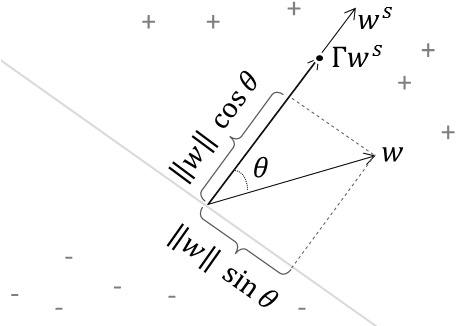
\includegraphics[scale=.6]{transfer/fig/pmt-svm.png}
	\caption{Projecting $w$ to $w'$ in PMT-SVM (adapted from \cite{aytar2011tabula}).}\label{fig:gama:pmt}
\end{figure}

Based on this, Projective Model Transfer SVM (PMT-SVM) is proposed to solve the transfer problem by optimizing the following objective function \cite{aytar2011tabula}:

\begin{equation}\label{eq:gama:pmt}
\begin{aligned}
\min \qquad& {L_{PMT}} = \frac{1}{2}{\left\| w \right\|^2} + \gamma {\left\| {Pw'} \right\|^2} + \frac{C}{2}\sum\limits_{i = 1}^l {\varepsilon _i^2} \\
\text{s.t.}\qquad&{y_i} = w{x_i} + b + {\varepsilon _i} \quad   \text{for} \quad i \in \left\{ {1,2,...,l} \right\}\\
& w^Tw' \ge 0
\end{aligned}
\end{equation}

Where $P$ is the the projection matrix $P = I - \frac{{w{'^T} \times w'}}{{w' \times w{'^T}}}$. Therefore, ${\left\| {Pw} \right\|^2} = {\left\| w \right\|^2}{\sin ^2}\theta $ is the
squared norm of the projection of the $w$ onto the source hyperplane (see Figure \ref{fig:gama:pmt}). As $\gamma \rightarrow 0$, the loss function \eqref{eq:gama:pmt} becomes a classic LS-SVM loss function. Because \eqref{eq:gama:pmt} is convex, it can be solved effectively by quadratic optimization.

In summary, both ASVM and PMT-SVM are designed to answer the question: how to transfer by solving some convex objective function. However, they both require a pre-defined parameter $\gamma$, which controls the amount of the knowledge to be transfered, to complete the objective function. In most cases, this parameter can only be set according to the background knowledge. Also, both methods can only adopt the knowledge from single source model which limits the their performance. 
\textbf{Multi-KT}
To learning from many sources, Multi Model Knowledge Transfer (Multi-KT) is proposed to reply on multiple sources by assigning different weight for each of them \cite{tommasi2014learning}. Similar to the objective function \eqref{eq:gama:asvm}, its objective function is defined as follow: 

\begin{equation}\label{eq:gama:multi}
\begin{aligned}
\min \qquad& {L_{Multi - KT}} = \frac{1}{2}{\left\| {w - \sum\limits_k {{\beta _k}} {{w'}_k}} \right\|^2} + \frac{C}{2}\sum\limits_{i = 1}^l {{\zeta _i}\varepsilon _i^2}  \\
\text{s.t.}\qquad&{y_i} = w{x_i} + b + {\varepsilon _i} \quad   \text{for} \quad i \in \left\{ {1,2,...,l} \right\}
\end{aligned}
\end{equation}
Here, $\beta_k$ is the weight assigned for the $k$th source model and $\zeta _i$ is defined as:

\begin{equation*}
{\zeta _i} = \left\{ {\begin{array}{*{20}{c}}
	{\frac{N}{{2{N^ + }}}}&{{\text{if }}{y_i} =1}\\
	{\frac{N}{{2{N^ - }}}}&{{\text{if }}{y_i} =- 1}
	\end{array}} \right.
\end{equation*}
where $N^+$ and $N^-$ are number of positive and negative examples respectively and $N$ is the total number of examples. 

The primal Lagrangian for optimization problem \eqref{eq:gama:multi} can be written as:
\begin{equation}
{L_{Multi - KT}}\left( {w,\beta ,\varepsilon ,\alpha } \right) = \frac{1}{2}{\left\| {w - \sum\limits_k {{\beta _k}} {{w'}_k}} \right\|^2} + \frac{C}{2}\sum\limits_{i = 1}^l {{\zeta _i}\varepsilon _i^2}  + \sum\limits_{i = 1}^l {{\alpha _i}\left[ {w{x_i} + b + {\varepsilon _i} - {y_i}} \right]} 
\end{equation}
So problem \eqref{eq:gama:multi} can be solved once $\beta$ is set.
Different from ASVM and PMT-SVM which require background knowledge to select proper transfer parameter, Multi-KT can estimate the transfer parameter $\beta$ itself by using the closed-form Leave-One-Out (LOO) error. According to \cite{cawley2006leave}, the closed-form LOO error is defined as:
\begin{equation}\label{eq:gama:loo}
{y_{i}} - {\hat y_{i}} = \frac{{{\alpha _{i}}}}{{\psi_{ii}^{ - 1}}}{\qquad\text{for}}\qquad i = 1,...,l
\end{equation}
Here $\psi_{ii}^{-1}$ is its $ith$ diagonal element of $\psi^{-1}$ in \eqref{eq:gama:psi}.

To estimate $\beta$, a loss function, similar to hinge loss, is defined as: 
\begin{equation}\label{eq:gama:multib}
\begin{aligned}
\text{min} \qquad&{\cal L} = \sum\limits_i^l {{\zeta _i}{{\left| {1 - {y_i}{{\hat y}_i}} \right|}_ + }} \\
\text{s.t.} \qquad& \left\| \beta  \right\| \le 1
\end{aligned}
\end{equation}

Here $|x|_+=max(x,0)$. Intuitively, if $\beta$ is properly set, ${y_i}{{\hat y}_i}$ should be positive for each $i$. However, focusing only on the sign of those quantities would result in a non-convex formulation with many local minima. By adding the $|\cdot|_+$ function, formula \eqref{eq:gama:multib} becomes convex and can be solved by gradient descent method.

\subsubsection{MULTIpLE}

MULticlass Transfer Incremental LEarning (MULTIpLE) focuses on adding a new class to an existing $N$ class source problem while preserving the performance on the old classes \cite{kuzborskij2013n}. To preserving the overall performance of the classifier among $N+1$ classes, MULTIpLE contains two parts: incremental learning for existing $N$ classes and transfer learning for the new class.

For the existing $N$ classes, MULTIpLE uses the similar strategy as ASVM, setting the transfer parameter $\gamma$ to 1. For the new class, it adopts the strategy of Multi-KT, combining knowledge from existing $N$-class models. As a result, the objective function for the hyperplanes in MULTIpLE is defined as:

\begin{equation}
\begin{aligned}
\text{min}\qquad {} & L_{MULTIpLE}=\frac{1}{2}\sum\limits_{n = 1}^N {{{\left\| {{w_n} - {{w'}_n}} \right\|}^2}}  + \frac{1}{2}{\left\| {{w_{N + 1}} - \sum\limits_{k = 1}^N {w{'_k}{\beta _k}} } \right\|^2}+ \frac{C}{2}\sum\limits_{n = 1}^{N + 1} {\sum\limits_{i = 1}^l {\varepsilon _{i,n}^2} }  \\
\text{s.t.}\qquad {} &{\varepsilon _{i,n}} = {Y_{in}} -  {x_i}{w_n} - {b_n}
\end{aligned}\label{eq:gama:multiple}
\end{equation}

Similar like Multi-KT, MULTIpLE uses LOO error in \eqref{eq:gama:loo} to estimate the transfer parameter $\beta$ for the new class. The objective function for $\beta$ estimation is defined by \cite{crammer2002algorithmic}:
\begin{equation}\label{eq:gama:multib}
\begin{aligned}
\text{min} \qquad& {\cal L}\left( {\beta ,i} \right) = \left\{ {\begin{array}{*{20}{c}}
	{\mathop {\max }\limits_{n \ne {y_i}} {{\left| {1 - {{\hat Y}_{in}}\left( \beta  \right) - {{\hat Y}_{i{y_i}}}\left( \beta  \right)} \right|}_ + }}&{{:y_i} \ne N + 1}\\
	{\left| {1 - {{\hat Y}_{in}}\left( \beta  \right) - {{\hat Y}_{i{y_i}}}\left( \beta  \right)} \right|}&{{:y_i} = N + 1}
	\end{array}} \right.  \\
\text{s.t.} \qquad& \left\| \beta  \right\| \le 1
\end{aligned}
\end{equation}
We can find the optimal $\beta$ with projected subgradient descent \cite{BoydCO}. 

These previous methods provided an approach to transfer the knowledge under the HTL setting. The previous methods try to use the hyperplane parameter as the transferable knowledge and thus limited to leverage the source knowledge from SVMs. In chapter \ref{sec:pakdd} of this thesis, we extend their methods and propose a novel method EMTLe under the HTL setting which can leverage the knowledge from more types of source models. 

\subsection{Distillation for Knowledge Transfer}
\textbf{Distillation} \cite{hinton2015distilling} was developed frameworks for knowledge transfer and addressed the problem how to effectively transfer the knowledge from the source model directly. In chapter \ref{sec:aaai}, we propose a framework called GDSDA based on it to solve semi-supervised domain adaptation problem. In this part, we review the principle of Distillation and some related work using this framework. The technical details will be introduced in chapter \ref{sec:aaai}.

Hinton et al. proposed Distillation to transfer the knowledge from a source neural network (or a whole ensemble of neural networks) to a single target one. In this setting, the capacity of the source neural network is large while the capacity of the target one is small. The capacity reflects the expressive power of a model and a model with larger capacity can fit complex data better. In statistical learning theory \cite{vapnik1999overview}, the relationship of the generalization error $e_{te}$ and training error $e_{tr}$ of a model can be expressed as follow:
\begin{equation}\label{eq:rw:general}
e_{te}\leq e_{tr}+2\sqrt{\frac{\log h +\log\frac{2}{\eta}}{2N}}
\end{equation}
Here, $h$ is the capacity (VC dimension) of the model and $N$ is the training set size. Inequation \ref{eq:rw:general} holds with a probability of $1-\eta$.
When we train the target model, we can let it mimick the output of the source one on the training set. If both source and target models can achieve similar training error on the training set, the small target model can typically do much better on the test data due to its lower capacity. In this process, we don't need the true label of the training data. Instead, we only require the outputs of the source model of the training data. The output of the source model is usually called the ``soft label". However, introducing the true label of the training data can further improve the performance of the target model. In distillation, imitation parameter is used to balance the importance between the soft label and true label.

Distillation is typically used for training the deep neural network for knowledge transfer between different models and tasks. Tzeng et al. \cite{Tzeng_2015_ICCV} proposed a CNN architecture for domain adaptation to leverage the knowledge from limited or no labeled data using the soft label. Urban et al. \cite{urban2016deep} use a small shallow net to mimick the output of a large deep net while using layer-wised distillation with $\ell_2$ loss of the outputs of student and teacher net. Similarly, Luo et al. \cite{luo2016face} use $\ell_2$ loss to train a compressed student model from the teacher model for face recognition. Gupta et al. \cite{Gupta_2016_CVPR} use supervision transfer to distil the knowledge from a trained CNN with unlabeled data or just a few labeled data.

In this thesis, we propose a novel framework that uses distillation for domain adaptation.
The limitation of the previous work in Distillation is that it is difficult to determine the value of the imitation parameter. Previous studies avoid this problem by either using brutal force searching or domain knowledge. To better solve this problem, we proposed a novel method that can autonomously balance the importance and extend it to the semi-supervised domain adaptation.





